\chapter{RAUFlow}

% **************************** Define Graphics Path **************************
\ifpdf
    \graphicspath{{Chapter5/Figs/Raster/}{Chapter5/Figs/PDF/}{Chapter5/Figs/}}
\else
    \graphicspath{{Chapter5/Figs/Vector/}{Chapter5/Figs/}}
\fi

En cap\'itulos anteriores se ha detallado las caracter\'isticas m\'as importantes del prototipo, as\'i como las principales componentes del router opensource y la entidad Controlador. 
Resta detallar entonces, el dise\~no de la aplicaci\'on que correr\'a en el dispositivo controlador y ser\'a encargada de implementar el plano de control; de aqu\'i en m\'as RauFlow. Por ello en el presente cap\'itulo se propone un an\'alisis de dicha componente, siguiendo un proceso de dise\~no tradicional de Ingenier\'ia de Software, dividido en 4 etapas. Una primera etapa de an\'alisis de requerimientos, una segunda etapa de relevamiento de casos de uso, una tercera etapa de dise\~no del modelo de datos, y finalmente una cuarta etapa para el dise\~no general de la arquitectura de la aplicaci\'on. Finalmente se presentan los aspectos m\'as importantes relacionados a la implementaci\'on de RAUFlow. 

\section[An\'alisi de requerimientos]{An\'alisis de requerimientos}

Anteriormente en ~\ref{section1.2.2} se definieron algunos de los requerimientos relevados para el prototipo de la RAU. De ellos y de un trabajo de an\'alisis sobre la realidad modelada, se desprende la siguiente tabla de requerimientos para RauFlow.

\clearpage
\begin{table}[Htl]\centering
\begin{tabularx}{\textwidth}{|>{\setlength\hsize{1.0\hsize}\setlength\linewidth{\hsize}}X|}
\hline
Requerimientos Funcionales\\ \hline
\hline
\begin{itemize}
\item El Sistema debe de proveer la facilidad para obtener la informaci\'on asociada a cada nodo de la red, permitiendo a su vez agregar informaci\'on que facilite la identificaci\'on del mismo para un usuario.
\item El Sistema debe proveer la facilidad para agregar, modificar y eliminar redes virtuales. 
%En particular al trabajar con redes virtuales y sus datos, se debe soportar el manejo de datos como la numeraci\'on IP del tr\'afico asociado a una red virtual, informaci\'on de capa de transporte, entre otros.
\item El Sistema debe proveer la facilidad para obtener toda la informaci\'on relevante de una red virtual.
\item El Sistema debe permitir visualizar de alguna forma los caminos constru\'idos para encaminar el tr\'afico de una red virtual en particular, a trav\'es de la red del protot\'ipo.
\item El Sistema debe proveer la facilidad para visualizar el estado de las tablas de flujos asociadas a cualquier nodo de la red del protot\'ipo.
\end{itemize}\\
\hline
\end{tabularx}
\end{table}

\begin{table}[Htl]\centering
\begin{tabularx}{\textwidth}{|>{\setlength\hsize{1.0\hsize}\setlength\linewidth{\hsize}}X|}
\hline
Requerimientos no Funcionales\\ \hline
\hline
\begin{itemize}
\item Se debe utilizar siempre que sea posible herramientas de software libre y c\'odigo abierto.
\end{itemize}\\
\hline
\end{tabularx}
\end{table}

Teniendo en cuenta la descripci\'on del problema y los requerimientos anteriores, se procedio con el modelado de la realidad. Los resultados obtenidos se presentan en la siguiente secci\'on.

%Teniendo en cuenta los requerimientos anteriores, se procede con el relevamiento de los casos de uso. Los resultados obtenidos se presentan en la siguiente secci\'on.

\section[Modelado de la realidad]{Modelado de la realidad}

En la figura ~\ref{fig:ModeloDeDominio} se presenta el modelo de dominio realizado a partir de la realidad planteada. En el mismo se destacan en color amarillo aquellas entidades que se entiende se corresponden al modelado de los elementos de la topolog\'ia como lo son Nodos e Interfaces. Por otro lado en rosado se destacan aquellas entidades relacionadas al concepto MPLS que se consideran importantes, como lo son las tablas FTN, ILM y NHLFE. Finalmente vale la pena destacar el concepto de Servicio, con el cual se decidi\'o representar a las redes virtuales soportadas en el protot\'ipo. Interesa destacar adem\'as del concepto de Servicio, que es una redefinici\'on desde una visi\'on centralizada del concepto FEC en la teor\'ia de MPLS, concepto que en la literatura de MPLS tradicional esta vinculado a un solo nodo en una red, y no a muchos como se propone en este trabajo.  

\begin{figure}[ht!] 
\centering    
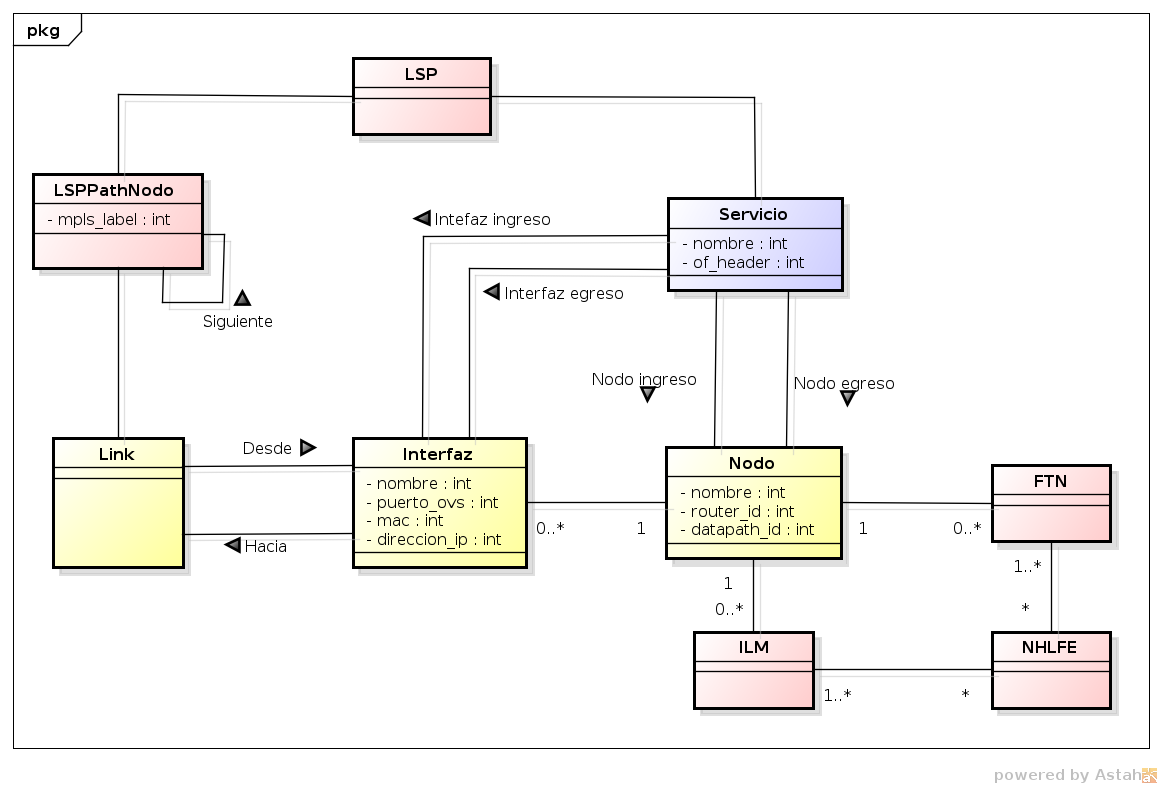
\includegraphics[width=0.7\textwidth]{Disenio_Figure1}
\caption[ModeloDeDominio]{Modelo de Dominio}
\label{fig:ModeloDeDominio}
\end{figure}

Sobre este modelo de dominio se trabaj\'o hasta llegar finalmente al diagrama de clase de dise\~no que se presenta a continuaci\'on en la figura [ref].\\

Teniendo en cuenta los requerimientos mencionados, y el modelado de la realidad presentado, se procede con el relevamiento de los casos de uso. Los resultados obtenidos se presentan en la siguiente secci\'on.

\section[Relevamiento de casos de uso]{Relevamiento de casos de uso}

La lista de casos de uso presentada a continuaci\'on se corresponde con un conjunto de funcionalidades b\'asicas, que permiten la exploraci\'on de la potencialidad del enfoque SDN aplicado al problema planteado. 

\begin{itemize}
\item Listar Servicios
\item Agregar Servicio
\item Modificar Servicio
\item Eliminar Servicio
\item Ver Topolog\'ia
\item Ver informaci\'on b\'asica Nodo
\item Ver tabla de Flujos Nodo
\item Filtrar Lsps
\item Editar Informaci\'on extra Nodo
\item Editar Informaci\'on extra Interfaz
\end{itemize}

De esta forma quedan presentados los requerimientos relevados sobre RauFlow, el modelado de la realidad, y los casos de uso relevados. Resta entonces presentar un esbozo de la arquitectura de la aplicaci\'on RauFlow, para que el lector finalmente este en condiciones de comprender el dise\~'no del prototipo en su totoalidad.

\section[Arquitectura de RauFlow]{Arquitectura de RauFlow}

En la figura ~\ref{fig:VistaComponentes2} se presenta un esquema con las componentes l\'ogicas que forman parte de la aplicaci\'on denominada RauFlow. Como se explico anteriormente, Ryu habilita la programaci\'on del plano de control mediante aplicaci\'ones desarrolladas en lenguaje Phyton con una cierta estructura particular. Por consiguiente RauFlow esta basado en al menos una aplicaci\'on de este tipo.\\

Por otro lado si bien Ryu ofrece un entorno para la ejecuci\'on de m\'ultiples aplicaciones, asi como un mecanismo para la comunicaci\'on entre ellas, por simplicidad se opto por basar el dise\~no de RauFlow en una \'unica aplicaci\'on Ryu lo m\'as simple posible. Luego funcionalidades y responsabilidades que no son previstas en dicha aplicaci\'on son implementadas por componentes adicionales, siguiendo un dise\~no modular.\\

Cabe destacar adem\'as, la existencia en el dise\~no de un conjunto de aplicaciones Ryu, dise\~nadas e implementadas por tereceros. Estas aplicaciones en particualr se encuentran dentro del conjunto de aplicaciones que vienen con el software Ryu. M\'as adelante se explicar\'a en detalle cual es el rol que cumplen estas aplicaciones en el dise\~no de RauFlow.\\

En relaci\'on a la arquitectura de RauFlow, esta se puede dividir en tres capas l\'ogicas; una capa de Presentaci\'on, una capa de Negocios y una capa de aplicaciones Ryu.

%En su dise\~no, RauFlow puede ser estudiado a trav\'es de 3 capas l\'ogicas. Comenzando por ejemplo por el estudio de una capa de Presentaci\'on y una capa Negocios, y terminando con el estudio de una capa de Aplicaciones Ryu.\\ 

%Esta \'ultima capa tiene sentido como tal, cuando el prototipo requiere de la ejecuci\'on de m\'ultiples aplicaciones Ryu, aspecto que ser\'a retomado m\'as adelante en esta secci\'on.\\

En la capa de aplicaciones Ryu, se encuentran los programas encargados de implementar los procesos y protocolos del plano de control. Dichas aplicaciones mantienen el dise\~no de una aplicaci\'on Ryu. Es en esta capa que se ubica la aplicaci\'on de Ryu encargada de implementar el plano de control, y que representa la escencia de RAUFlow.

Por otro lado, toda l\'ogica de negocios asociada a la realidad modelada se encuentra en la capa de Negocios, desacoplada totalmente de dicha aplicaci\'on. Esto obedece a un criterio de dise\~no en el cual se busca mantener la l\'ogica de la aplicaci\'on de Ryu lo m\'as simple posible, haciendola responzable principalmente por los eventos asociados al protocolo OpenFlow.\\ 

\begin{figure}[ht!] 
\centering    
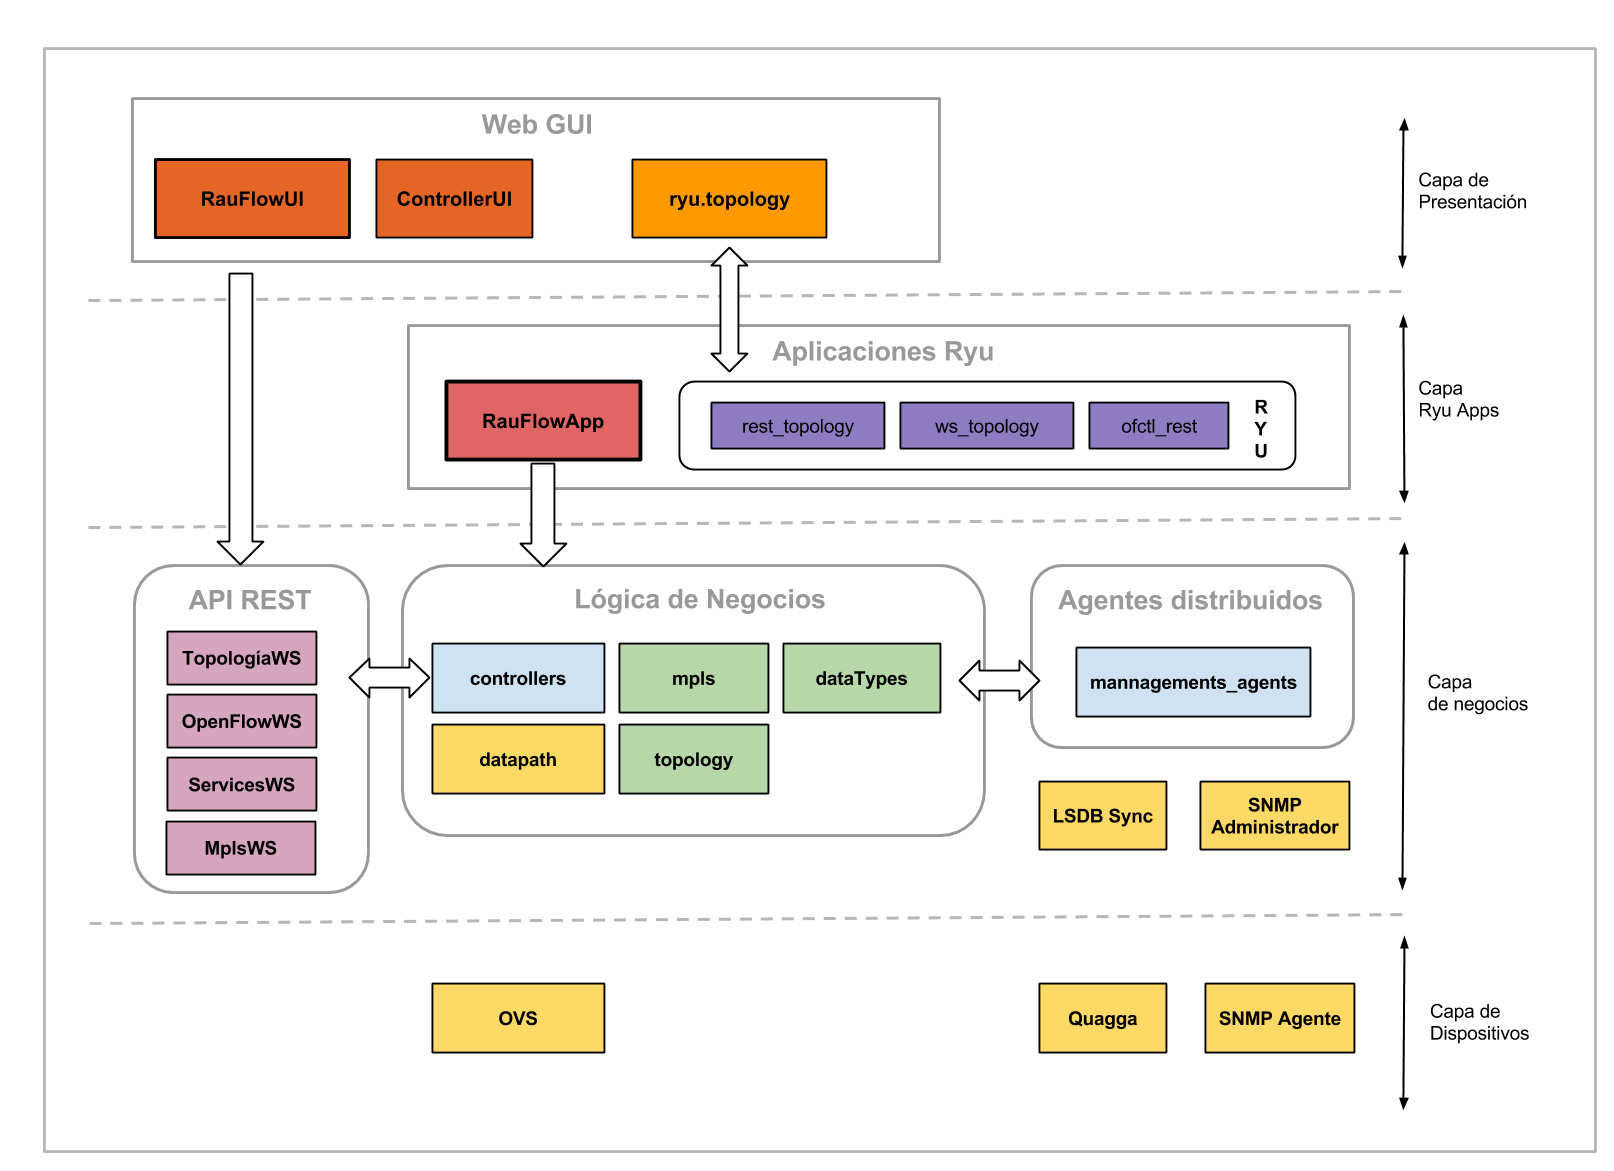
\includegraphics[width=1.0\textwidth]{Disenio_Figure3}
\caption[Vista l\'ogica]{Vista l\'ogica}
\label{fig:VistaComponentes2}
\end{figure}

Luego, en la capa de negocios se encuentran tres componentes. Una componente de l\'ogica de negocios, puramente relacionada a la realidad modelada, una API REST de servicios para el acceso y la manipulaci\'on de datos relacionados a la primera componente, y finalmente una tercera componente denominada Agentes distribu\'idos.\\

Profundizando en la componente de l\'ogica de negocios, esta se encuentra a su vez sub-dividida en diferentes m\'odulos que agrupan funcionalidades acorde a su naturaleza y responsabilidades. De estos m\'odulos vale la pena destacar el m\'odulo \textbf{topology} responsable de la representaci\'on de la topolog\'ia y las operaciones para la manipulaci\'on de la misma, el m\'odulo \textbf{mpls} responsable por las operaciones y conceptos relacionados al protocolo mpls, y el modulo \textbf{datapath} responsable del acceso y manipulaci\'on de los diferentes dispositivos de la red.\\ 

Por otro lado, enfocandose en la componente de Servicios REST, la misma se encuentra sub dividida en varios m\'odulos respondiendo al criterio utilizado para el dise\~no modular de la componente de l\'ogica de negocios. Dicha componente comprende desde un modulo de servicios para el acceso a la informaci\'on de la topolog\'ia, un modulo de servicios para el acceso a la informaci\'on relacionada a mpls, hasta un m\'odulo de servicios para el acceso a informaci\'on de naturaleza OpenFlow vinculada a los diferentes dispositivos del datapath.\\

Finalmente, en relaci\'on a la componente denominada Agentes distribu\'idos, esta se encarga de la interacci\'on con diferentes agentes y procesos instalados en cada router opensource a traves de un canal IP. Este m\'odulo de comunicaci\'on, as\'i como los diferentes agentes instalados en cada router opensource, juegan un rol irremplazable en la obtenci\'on de informaci\'on; puesto que a partir del canal de comunicaci\'on OpenFlow solamente es accesible Open vSwitch y la informaci\'on contemplada por el protocolo OpenFlow.

Dentro de esta componente, en el diagrama se muestra un modulo denominado \textbf{managements\_ agents}. Este m\'odulo opera como una interfaz de conexi\'on entre los diferentes m\'odulos de la l\'ogica de negocios, y los diferentes m\'odulos que implementan la comunicaci\'on con su respectivo agente distribu\'ido.

En la figura ~\ref{fig:VistaComponentes2} se muestran el modulo \textbf{SNMP Management}, responsable de  la comunicaci\'on con un agente SNMP distribu\'ido entre los nodos del prototipo, con el fin de obtener informaci\'on extra acerca de las interfaces de red de cada router opensource.\\

De esta forma se llega a la capa de presentaci\'on. En la misma se destacan: una interfaz gr\'afica identificada en el esquema como RauFlowUI, la cual implementa cada uno de los casos de uso mencionados anteriormente en [link a la secci\'on de casos de uso], otra componente identificada como ControladorUI la cual funciona a como nexo entre las funcionalidades de RauFlowUI y la API Rest de Servicios, y la componente identificada como \textbf{ryu.topology}. Esta \'ultima componente forma parte del conjunto de apliaciones Ryu adicionales que se incluyen en el dise\~no de RauFlow, y tiene como principal funci\'on la de proveer una representaci\'on gr\'afica en tiempo real de la topolog\'ia existente en el prototipo.\\

Habiendose explicado en detalle cada una de las capas l\'ogicas en el dise\~no de RauFlow, se aborda a continuaci\'on las aplicaciones Ryu desarrolladas por terceros.\\

Ryu incluye tres aplicaciones dise\~nadas para implementar una interfaz gr\'afica. Dicha interfaz consiste en un p\'agina web implementada sobre html, javascript y web sockets, que permite visualizar la red en su totalidad. Estos son los dispositivos del datapath con sus interfaces, y los enlaces existentes.

Por esta razon se incluyen en el dise\~no del proptotipo dichas aplicaciones, agregando funcionalidades  a la capa de presentaci\'on, y reutilizando desarrollos existentes.

%que permite visualizar de forma similar a un grafo los diferentes deispositivos del datapath.

%Deacuerdo con los objetivos de este proyecto, el desarrollo de una interfaz gr\'afica no esta necesariamente inclu\'ido dentro del alcance final. De todas formas se incluye el desarrollo de la misma como un objetivo de baja prioridad puesto que agrega valor al prototipo final. Por otro lado dentro del conjunto de aplicaciones que trae el controlador Ryu, se incluyen tres aplicaciones que ejecutandose en conjunto con una aplicaci\'on web, proporcionan una interfaz gr\'afica, cuya \'unica funcionalidad es la de mostrar la topolog\'ia actual de red mediante un grafo. Adem\'as vale la pena destacar que esta implementada en base a web sockets, por lo que la vista topol\'ogica se mantiene constantemente actualizada.\\

\section[Implementaci\'on]{Implementaci\'on}

En esta secci\'on se presentan los aspectos m\'as importantes en relaci\'on a la implementaci\'on de RauFlow.\\

[AYUDA MEMORIA: Cosas de las que hay que hablar]

\begin{itemize}
\item SPF y CSPF: Mostrar el pseudo codigo del algoritmo de ruteo implementado, mencionar que esta construido sobre dijkstra para multigrafos. En particular mencionar que cosas de QoS interesaria meter en este algoritmo para garrantizar QoS despues en RauFlow

\item Mencionar como se implementaria QoS en RauFlow

\item Capaz algo sobre la interfaz 
\end{itemize}